\subsection{射影线性簇}

每个单射线性映射 \(f\) ——\(\mathbf{R}^{n+1}\) 到 \(\mathbf{R}^{m+1}\) 中的（ \(m \geqslant n\) ）——通过限制到 \(\mathbf{R}_{n+1}^*\) 再关于关系 \(\Delta_n\) 与 \(\Delta_m\) 取商（《集合论》，R，§ 5，第 8 小节），定义了一个单射映射 \(g\) ——\(\mathbf{P}_n\) 到 \(\mathbf{P}_m\) 中的——，称为射影线性映射。若 \(\varphi\) （相应地，\(\psi\)）是 \(\mathbf{R}_{n+1}^*\) 到 \(\mathbf{P}_n\) 上（相应地，\(\mathbf{R}_{m+1}^*\) 到 \(\mathbf{P}_m\) 上）的典范映射，则我们有 \(g \circ \varphi = \psi \circ f\) ，这表明 \(g\) 在 \(\mathbf{P}_n\) 上连续（第 I 章，§ 3，第 4 小节，命题 6 的推论）。特别地，\(\mathbf{P}_n\) 的每个射影线性变换（即 \(\mathbf{P}_n\) 到其自身的射影线性映射）是 \(\mathbf{P}_n\) 到其自身的一个同胚。

我们还回忆，若 V 与 \(V'\) 是两个 p 维射影线性簇（\(P_{n}\) 中的），则存在 \(P_{n}\) 的一个射影线性变换把 V 变换为 \(V'\)。特别地，若 \(p \geqslant 0\) ，则存在把 V 变换成坐标射影线性簇的射影线性变换，也就是说，变换成坐标簇 \(W'\) （\(p + 1\) 维的，\(R^{n+1}\) 的，去掉点 o 的）的典范象。若把 \(W'\) 与 \(R_{p+1}^{*}\) 等同，\(\Delta_{n}\) 在 \(W'\) 上诱导的关系正是 \(\Delta_{p}\) ；由于 \(W'\) 是闭的且关于 \(\Delta_{n}\) 饱和，引理 1 表明 \(V'\) 同胚于 \(P_{p}\) 且在 \(P_{n}\) 中是闭的；此外，若 p \textless{} n，它的补集在 \(P_{n}\) 中稠密（§ 1，第 4 小节，命题 3 的推论）。因此：

命题 4. 射影空间 \(P_{n}\) 中每个 p 维射影线性簇在 \(P_{n}\) 中是闭的，且同胚于 \(P_{p}\)；若 p \textless{} n，其补集在 \(P_{n}\) 中稠密。

这个结果是在任意除环上的射影空间中把一维与二维射影线性簇称为射影直线与射影平面这些名称的由来。我们还回忆，\(P_{n}\) 中 n - 1 维的射影线性簇称为射影超平面；每个射影超平面等同于齐次坐标满足形如 \(\sum_{i=0}^{n}a_{i}x_{i}=0\) 的关系（其中诸 \(a_{i}\) 不全为零）的点所成的集（超平面的“方程”）。

\pandocbounded{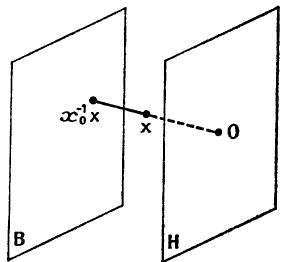
\includegraphics[keepaspectratio]{images/part001_d597a17f.jpg}}\\
图 4.

命题 5. 在射影空间 \(\mathbf{P}_n\) （ \(n \geqslant 0\)）中，射影超平面 H 的补集同胚于 \(\mathbf{R}^n\)。

作一个射影线性变换，我们可以假设 H 是方程为 \(x_{0}=0\) 的超平面。集 A ——由点 \(\boldsymbol{x}=(x_{i})\) （\(R_{n+1}^{*}\) 的，满足 \(x_{0}\neq0\) 的）组成——是开的且关于 \(\Delta_{n}\) 饱和；它的典范象 C （在 \(P_{n}\) 中的）——即 H 在 \(P_{n}\) 中的补集——因此同胚于 A 关于等价关系 \(\Theta\) （由 \(\Delta_{n}\) 在 A 上诱导的）的商（引理 1）。令 B 是方程为 \(x_{0}=1\) 的超平面（\(R^{n+1}\) 中的）。对每一点 \(x\in A\) ，使它对应于点 \(x_{0}^{-1}x\) ，即过 o 与 x 的直线和 B 的交点（图 4）；这样我们定义了 A 到 B 上的连续映射 g，使 \(g(x)\) 是 B 中与 x 模 \(\Theta\) 同余的唯一的点。由此推出 B 同胚于 A/ \(\Theta\) （引理 2），从而同胚于 C；由于 B 同胚于 \(R^{n}\) ，证明完成。

推论. \(P_{n}\) 的每个点都有一个同胚于 \(R^{n}\) 的开邻域。特别地由此推出实射影空间是局部连通的（这也可由第 I 章，§ 11，第 6 小节，命题 12 得出）。

